% FinalCheatSheetGPT.tex
\documentclass[11pt]{article}
\usepackage[margin=1in]{geometry}
\usepackage[hidelinks]{hyperref}
\usepackage{graphicx}
\usepackage{amsmath,amssymb}
\usepackage{longtable}
\usepackage{booktabs}
\usepackage{enumitem}
\usepackage{imakeidx}
\makeindex
\title{Final Cheat Sheet --- CSE508}
\author{Converted from FinalCheatSheet.md}
\date{May 11, 2026}

\begin{document}
\maketitle
\tableofcontents
\clearpage

% Overview
\section{Overview}
\index{Overview}
Confidentiality --- data is only accessible to authorized parties.\\
Integrity --- data has not been tampered with or corrupted during transit.\\
Anonymity --- hide the identity of the participants of the communication.

% Diffie-Hellman
\section{Diffie--Hellman}
\index{Diffie-Hellman}
\begin{itemize}
  \item DLP (Discrete Logarithm Problem): given $g^a$, find $a$.
  \item CDH (Computational Diffie--Hellman): given $g^a$ and $g^b$, compute $g^{ab}$.
  \item DDH (Decisional Diffie--Hellman): given $g^a,g^b$ and value $Z$, decide whether $Z=g^{ab}$ or random.
\end{itemize}

% OTP
\section{One--Time Pad (OTP)}
\index{One-Time Pad}
\begin{itemize}
  \item Encrypt: ciphertext = plaintext XOR key (key length = message length).
  \item Perfect secrecy if: key is truly random, used only once, and kept secret.
  \item Danger: key reuse — XOR of two ciphertexts cancels the key and leaks information.
\end{itemize}

% RSA
\section{RSA}
\index{RSA}
\subsection*{Key Generation and Use}
\begin{enumerate}
  \item Select two primes $p$ and $q$ and compute $n=pq$.
  \item Choose $e,d$ such that $ed\equiv1\pmod{\phi(n)}$.
  \item Public key $(e,n)$, private key $(d,n)$.
  \item Encryption: $c\equiv m^e\pmod n$. Decryption: $m\equiv c^d\pmod n$.
\end{enumerate}
\noindent Note: RSA is deterministic without padding and requires OAEP (or similar) for IND-CPA; quantum algorithms threaten RSA.

% AES modes
\section{AES Modes}
\index{AES}
\subsection*{ECB}
Independent block encryption; deterministic and leaks patterns — avoid for multi-block plaintexts.

\subsection*{CBC}
Uses IV and chaining; encryption $C_i=E_K(M_i\oplus C_{i-1})$; needs integrity protection; vulnerable to padding oracles if padding validity is observable.

\subsection*{CTR}
Stream-like with counter/nonce: $C_i=M_i\oplus E_K(IV+i)$. Nonce reuse under same key is catastrophic.

\subsection*{AEAD (GCM/CCM)}
Provides authenticated encryption (confidentiality + integrity). Use AEAD (e.g. AES-GCM, ChaCha20-Poly1305) when possible.

% Merkle tree
\section{Merkle Tree}
\index{Merkle Tree}
Hash leaves, iteratively hash pairs to compute the Merkle root which commits to all data blocks.

% Common Weaknesses
\section{Common Weaknesses}
\index{Weaknesses}
\begin{longtable}{p{0.28\linewidth} p{0.34\linewidth} p{0.34\linewidth}}
\toprule
\textbf{Weakness} & \textbf{Typical attack} & \textbf{Mitigation} \\
\midrule
Static keys & Retrospective decryption & Use ephemeral keys (Perfect Forward Secrecy) \\
No randomness & Replay attacks & Use nonces, sequence numbers, timestamps \\
Weak hashing & Collision attacks & Use SHA-256 or stronger \\
Plaintext handshake & Eavesdropping & Use modern TLS (encrypted handshake) \\
\bottomrule
\end{longtable}

% Information Flow & Side-channels
\section{Information Flow \& Side-channels}
\index{Information Flow}
Noninterference: secret (High) inputs should not affect public (Low) outputs. Covert channels (timing, resource usage) and side-channels (timing, cache, power) leak secrets. Defenses: constant-time code, blinding, reduce observable state, limit timer precision, uniform error handling.

% CBC Padding Oracle
\section{CBC Padding Oracle (Vaudenay / Lucky13)}
\index{Padding oracle}
PKCS\#7 padding uses p bytes of value p; padding validation responses or timing differences enable adaptive attacks (Vaudenay). Lucky13 exploited timing differences in MAC+padding processing. Mitigations: use AEAD, encrypt‑then‑MAC, constant‑time checks, and indistinguishable error messages.

% Privacy, Tor
\section{Privacy, Anonymity \& Tor}
\index{Privacy}
Privacy controls collection/use of PII; anonymity prevents linking actions to identities. Fingerprinting (canvas, WebGL, fonts, AudioContext) and website fingerprinting (packet timing/size) can deanonymize users.

Mixnets add batching and reordering (high latency, strong anonymity). Tor uses onion routing: entry guards, middle relays, exit nodes; hidden services use introduction/rendezvous points and DHT descriptors. Operational tips: use Tor Browser, reduce fingerprinting surface, avoid mixing sensitive destinations on same circuits, use entry guards, consider traffic shaping/padding for higher anonymity.

% DNS
\section{DNS Protocol Recap}
\index{DNS}
Resolver flow: stub resolver $\rightarrow$ recursive resolver $\rightarrow$ root $\rightarrow$ TLD $\rightarrow$ authoritative server. Transport: UDP/53 (default), TCP/53 (truncation/AXFR), DoT/DoH for encrypted queries. Important RRs: A, AAAA, NS, CNAME, MX, PTR, TXT, SOA. Use EDNS(0), DNS Cookies, QNAME minimization.

\subsection{DNSSEC}
\index{DNSSEC}
Digitally signs records with chain of trust (root→TLD→authoritative). Provides integrity and origin authentication but not confidentiality.

\begin{figure}[h]
  \centering
  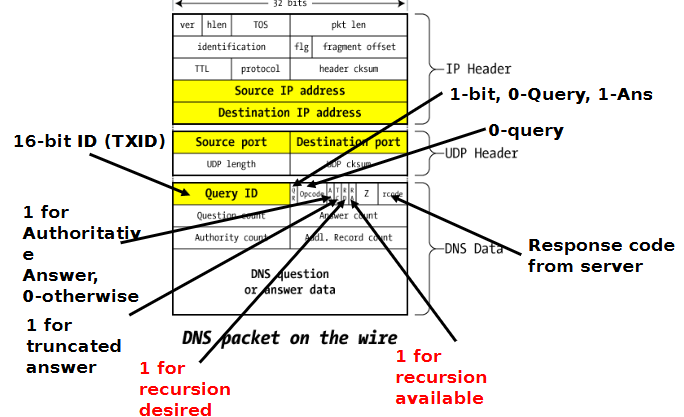
\includegraphics[width=0.6\textwidth]{media/DNSPacket.png}
  \caption{DNS packet (illustrative)}
\end{figure}

\subsection{CDN (Content Delivery Network) \& DNS}
\index{CDN}
CDNs use DNS (geo‑DNS / EDNS client subnet) or HTTP redirects to point clients to nearby PoPs (edge servers). Flow: resolver → CDN authoritative DNS → returns IP for best PoP (may use ECS). TTLs short. Benefits: caching, reduced origin load, improved latency, DDoS absorption. Risks: DNS compromise or cache poisoning can redirect users; EDNS client subnet leaks partial client location. Mitigations: protect authoritative DNS (DNSSEC, Anycast), use CDN WAF/DDoS, monitor edge health.

% SSL/TLS
\section{SSL/TLS}
\index{TLS}
Purpose: confidentiality, integrity, endpoint authentication for application protocols. TLS 1.3 uses ECDHE, AEAD, encrypted handshake messages, PSK/tickets for resumption, optional 0-RTT.

\subsection{TLS 1.3 (1-RTT overview)}
\begin{enumerate}
  \item ClientHello sends supported suites and KeyShare.
  \item ServerHello selects suite and returns KeyShare.
  \item Encrypted handshake messages: EncryptedExtensions, Certificate, CertificateVerify, Finished.
  \item Client verifies Certificate and sends Finished.
\end{enumerate}

Key features: ephemeral ECDHE for PFS, AEAD ciphers for auth+enc, session resumption via PSK, 0-RTT replay risk.

\subsection{Vulnerabilities and mitigations}
Misissued CAs, downgrade attacks, implementation bugs, 0-RTT replay. Mitigate: prefer TLS 1.3, disable legacy ciphers, enable AEAD, constant-time processing, OCSP stapling, short-lived certs.

% FTP
\section{FTP (File Transfer Protocol)}
\index{FTP}
Plaintext by default: control channel TCP/21 sends commands and credentials cleartext unless FTPS or SFTP used.

Active vs Passive modes:
\begin{itemize}
  \item Active (PORT): server connects back to client — problematic with NAT/firewall.
  \item Passive (PASV): server opens ephemeral data port; client connects — better for NATed clients.
\end{itemize}

Security: prefer FTPS (FTP over TLS) or SFTP (over SSH). Disable anonymous access, require strong auth, restrict data port ranges and firewall, log transfers, chroot users.

% Certificate Transparency & ACME
\section{Certificate Transparency (CT) \& ACME}
\index{Certificate Transparency}
CT: public append-only logs of issued certificates. CAs submit certs and provide Signed Certificate Timestamps (SCTs). Monitors watch logs for misissuance.

ACME: Automated Certificate Management Environment (Let's Encrypt). ACME flow:
\begin{enumerate}
  \item Client registers an account key.
  \item Client submits an order for a domain.
  \item Server returns authorization object with challenge options.
  \item Client fulfills a challenge (HTTP-01, DNS-01, TLS-ALPN-01).
  \item Server validates challenge; authorization marked valid.
  \item Client submits CSR; server issues certificate.
\end{enumerate}

ACME challenge tradeoffs (summary): HTTP-01 easy but no wildcard support and requires port 80; DNS-01 supports wildcards and internal servers but requires DNS API access and may suffer propagation delays.

\begin{table}[h]
\centering
\begin{tabular}{l p{0.4\linewidth} p{0.4\linewidth}}
\toprule
Challenge & Pros & Cons \\
\midrule
HTTP-01 & Easy to automate; works on standard port 80 & No wildcard support; requires inbound port 80 \\
DNS-01 & Supports wildcards; works for internal/private servers & Requires DNS API automation; DNS propagation delays \\
\bottomrule
\end{tabular}
\caption{ACME challenge comparison}
\end{table}

% DoS
\section{Denial-of-Service (DoS)}
\index{DoS}
Categories: volumetric/amplification (Smurf, DNS/NTP amplification), transport/state exhaustion (SYN flood), application-layer (Slowloris). Mitigations: upstream filtering, Anycast/CDN, SYN cookies, rate limiting, WAFs, blackholing.

\subsection{Smurf Attacks}
\index{Smurf attack}
Attacker spoofs victim IP and sends ICMP Echo to broadcast address; many hosts reply to victim causing amplification. Mitigate: disable IP-directed broadcasts, configure hosts to ignore broadcast ICMP, ingress filtering/uRPF.

% Firewalls & Tunnels
\section{Firewalls \& Tunnels}
\index{Firewalls}
Types: stateless ACLs, stateful firewalls, NGFW with L7 inspection. Rule order: allow RELATED,ESTABLISHED → allow required services → default-deny. Pitfalls: open management ports, UPnP, misordered rules, broad CIDRs.

\subsection{UPnP}
\index{UPnP}
UPnP allows LAN apps to request NAT port mappings, often unauthenticated on consumer gateways — malware can open WAN-accessible ports. Mitigate: disable UPnP, use manual port forwarding, restrict to trusted LAN, patch firmware, monitor dynamic mappings.

\subsection{Tunnels and VPNs}
\index{Tunnels}
SSH tunneling, IPSec (transport/tunnel modes), OpenVPN, WireGuard. Use strong auth, PFS, encrypt control and data planes, and apply NAT traversal (NAT-T) when needed.

\subsection{Zero Trust (brief)}
\index{Zero Trust}
"Never trust, always verify": authenticate & authorize each request, device posture checks, least privilege, microsegmentation, continuous telemetry.

\subsection{L2 vs L3 boundaries}
\index{L2/L3}
L2 (VLANs, switches) for local segmentation; vulnerable to ARP spoofing and CAM floods. L3 (routing, firewalls) enforces inter-VLAN policies and reduces broadcast domains. Combine: L2 isolation + L3 policy enforcement + microsegmentation.

\subsection{SSH Tunneling (conceptual)}
\index{SSH tunneling}
SSH tunneling uses an authenticated, encrypted SSH connection as a generic transport to carry other TCP connections or proxy traffic. When outbound SSH is allowed, encapsulating traffic inside the SSH session lets clients reach otherwise blocked destinations: the firewall only sees an allowed SSH session. Types: local forwarding, remote forwarding, dynamic proxying. Security: SSH server becomes an exit point — enforce strong auth (keys), restrict forwards, monitor.

% BGP
\section{BGP (Border Gateway Protocol)}
\index{BGP}
BGP runs over TCP/179; messages: OPEN, UPDATE, KEEPALIVE, NOTIFICATION. Route selection simplified: local-pref, AS_PATH length, origin type, MED, prefer eBGP, IGP distance. Risks: prefix hijacks, route leaks, AS_PATH manipulation. Mitigations: prefix filtering, max-prefix, RPKI/ROA, neighbor auth, monitoring (BGPmon).

\subsection{eBGP vs iBGP}
\index{eBGP}
\index{iBGP}
 eBGP between ASes (adjacent peers); iBGP within AS (requires full mesh or route reflectors).

% MAC vs Digital Signature
\section{MAC vs Digital Signature}
\index{MAC}
\index{Digital Signature}
\begin{tabular}{l l l}
\toprule
Feature & MAC & Digital signature \\
\midrule
Key type & Symmetric (shared secret) & Asymmetric (public/private) \\
Speed & Very fast & Slower (public-key ops) \\
Non-repudiation & No & Yes \\
Primary use & Message integrity & Non-repudiation / code signing \\
\bottomrule
\end{tabular}

% Short Practical Notes
\section{Short Practical Notes}
\index{Practical Notes}
Prefer ephemeral per-session keying for forward secrecy. Use AEAD when possible, ensure good randomness and key management. For network security QA, understand tradeoffs (speed vs non-repudiation) and appropriate uses of AEAD vs separate MAC+enc.

% In Class Highlights & Lecture extras
\section{In-Class Highlights}
\index{Lecture highlights}
Quick notes: Firewall ACLs and ordering, UPnP caveats, segmentation best practices.

\section{Lecture Extras}
\index{Lecture extras}
\begin{itemize}
  \item ARP poisoning/spoofing: inject fake ARP replies to poison caches → MITM. Defenses: static bindings, Dynamic ARP Inspection (DAI), monitoring.
  \item DHCP exhaustion/rogue DHCP: consume IP pool or provide bad config → mitigations: DHCP snooping, trusted ports, rate limits.
  \item MAC/CAM table flooding: overflow CAM to force fail-open → mitigations: port security, MAC limits.
  \item Wi‑Fi deauth & evil‑twin: spoof deauth or run rogue APs → mitigations: 802.11w (MFP), WPA2/3, AP authentication.
  \item "Evil packet" exploits (Ping-of-Death, LAND, Teardrop): crafted packets that crash stacks → patching, ingress filtering, fragmentation checks.
\end{itemize}

% PKI
\section{Public Key Infrastructure (PKI)}
\index{PKI}
Purpose: bind public keys to identities using X.509 certificates. CA hierarchy: Root → Intermediates → End-entity. Certificate fields: Subject, SAN, Issuer, Validity, Public Key, Signature, Extensions (keyUsage, EKU, basicConstraints, CRL/OCSP endpoints). Revocation: CRL, OCSP, OCSP stapling. Validation checklist: chain verification, expiry, CN/SAN match, keyUsage/EKU, revocation status. Threats: misissued/compromised CAs — mitigate with CT, HSMs, short-lived certs, auditing.

% End
\clearpage
\printindex
\end{document}
